\documentclass[]{article}

\usepackage{graphicx} %for å inkludere grafikk
\usepackage{verbatim} %for å inkludere filer med tegn LaTeX ikke liker
\usepackage{tabularx}
\usepackage{booktabs}
\usepackage{amsmath}
\usepackage{float}
\usepackage{color}
\usepackage{listings}
\usepackage{physics}
\usepackage{hyperref}
\usepackage{subfig}
\usepackage{mhchem}
\usepackage{natbib}
%opening
\title{}
\author{}

\begin{document}
	
\title{FREYA Report after Berkeley visit}
\author{Dorthea Gjestvang}
\date{January 2018}

\maketitle

\section{Introduction}

\section{Theory: FREYA}
FREYA is short for Fission Reaction Yield Algorithm, and it is a computer code that models fission of some nuclei \cite{FREYAusemanual}. In a fission event in FREYA, the energy, angular momentum and of the fragments and the emmited photons and neutrons are calculated, and thus it is possible to look at different aspects of the fission process using the same model. The calculations in FREYA are based on experimental data \cite{FREYAusemanual}, and today it can model spontaneous fission, photofission and neutron-induced fission for some given nuclei.

\subsection{Fission event in FREYA}

The simulation of a fission event in FREYA proceeds in several steps: pre-fission, during fission and post-fission, and I will focus on those aspects of the process that are of the most importance for this report. FREYA only concider the fission event, and the neutron and gamma emission from the pre-equilibrium nucleus, the compound nucleus and the fission fragments, and it does not take into account further decay of the fission products.

First, FREYA conciders the pre-equilibrium nucleus, and the chance for pre-equilibrium neutron emission. This is only significant for high energies \cite{FREYAusemanual}. Furthermore, the code conciders pre-fission neutron evaporation, where a neutron is emmited before fission occurs. The resulting $A-1$-nuclei has then a chance to fission, or emit another neutron. As each resulting nuclei can either emit a pre-fission neutron or fission, this process is called multichance fission. {citation needed}

After pre-fission radiation, FREYA moves on to the fission process. Using a energy-dependent fission fragment distribution, the mass numbers of the two fragments are decided, and the charge is split in accordance to a probability distribution \cite{FREYAusemanual}. The total mass number A and the charge Z is conserved in the fission process.

Now the energy of the fission fragments are to be determined. FREYA relies on experimental data to input the total kinetic energy TKE of the fission fragments for a given compound nuclei excitation energy \cite{FREYAusemanual}. By calculating the Q-value of the fission reaction and subtracting the average TKE, the energy available as excitation energy for the two fragments are found. This energy is first split between rotational and statistical excitation energy, and then split between the two fragments. The energy of the system is conserved. 

The last part of the FREYA fission event is the post-fission radiation, which consist of neutron and photon emission. First, the fission fragments emit neutrons until their statistical excitation energy is below the neutron separation energy, and neutron emission is no longer possible. Then the photon emission starts, beginning as a statistical cascade of photons. First the statistical excitation energy of the fission fragment is disposed of, then when the statistical excitation energy drops below a givel limit $g_{min}$, the emission of photons conntinues, now exhausting the rotational energy of the nucleus. This is colllective, discrete transitions between theoretical rotational bands in the nucleus. At low energies the photon emission continues as discrete transitions, using data from the RIPL-3 library \cite{FREYAusemanual}. When the remaining excitation energy is belov the limit $g_{min}$, or the nucleus has an half-life longer than the limit $t_{max}$, the process stops. FREYA has now simulated a complete fission event.

\subsubsection{Parameters in FREYA}
\label{Parameters_FREYA}
There are several adjustable parameters in FREYA, that enables the user to fit the calculations to experimental results. I will focus on a few of these that are important for this report. 

As mentioned earlier, the total kinetic energy of the fragment $TKE_{data}$ is needed as input in FREYA. FREYA further assumes that the avergage total kinetic energy takes the following form \cite{FREYAusemanual}:

\begin{equation}
	\label{eq:total_kinetiv_energy}
	TKE(A_H, E_n) = TKE_{data}(A_H) + dTKE(E_n)
\end{equation}

dTKE is an adjustable parameter, used to reproduce the measured average neutron multiplicity $\nu$. As the excitation energy E is TKE subtracted from Q, the dTKE-parameter adjusts the ratio of kinetic enery and excitation energy in the nucleus. \par 
\vspace{3mm}

The parameter c$_s$, called the spin temperature, adjusts the ratio between the fragment's rotational and statistical exitation energy. The angular momentum of the nucleus is drawn from a Boltzmann distribution, where c$_s$ is the factor that determines the temperature of the Boltzmann distribution. For c$_s = 1$ the angular momentum is drawn from a thermal distribution, and the higher the c$_s$, the higher probability of nuclei with high angular momentum. Thus, the higher c$_s$, the less statistical excitation energy will the fragments get. /par 

\vspace{3mm}

Observations show that statistical excitation energy is not shared evenly between the light and the heavy fission fragment, but rather that the lighter fragment is favoured \cite{FREYAusemanual}. The parameter x $>1.0$ shifts the statistical excitation energy to the light fragment by a fraction of x. A higher x will thus give the light frament a larger portion of the available statistical excitation energy.

\section{Method}

This report is based on work done with FREYA v2.0.3. Each case was run with 100000 iteratations, and with default parameters provided by FREYA, unless otherwise specified. 

The first case analysed was the spontaneous fission of Cf252. The dependence of the mean neutron multiplicity $\nu$, the mean neutron multiplicity from the light  and heavy fissions fragment $\nu_1$ and $\nu_2$, and the mean gamma multiplicity $N_{\gamma}$

\section{Results}

\subsection{Spontaneous fission of Cf252 }

The four first neutron factorial moments is shown in table \ref{tab:Cf252_n_moments}, and the dependence of the mean neutron multiplicity $\nu$ and the photon multiplicity $N_{\gamma}$ on the parameters dTKE and x  can be seen in Table \ref{tab:dependence_on_dTKE} and \ref{tab:dependence_on_x} respectively. The dependence of $N_{\gamma}$ on $c_s$ is shown in Table \ref{tab:dependence_on_c}.

The fragment and product mass distribution is shown in Figure \ref{fig:Cf252_sf_fragment_product_yield}, and the mean kinetic energy of the fragments as a function of mass is shown in Figure \ref{fig:Cf252_sf_mean_fragment_kinetic_enery_function_of_fragment_mass_number}. The multiplicity distribution and spectral shape of the emmited neutrons and photons respectively is shown in Figure \ref{fig:Cf252_sf_total_n_mult}, \ref{fig:Cf252_sf_neutron_spectral_shape}, \ref{fig:Cf252_sf_total_ph_mult} and \ref{fig:Cf252_sf_photons_spectral_shape}. The angular correlation between pairs of emmited neutrons are shown in Figure \ref{fig:Cf252_sf_n_n_ang_corr}.


\begin{table} [H]
	\centering
	\caption{The four first neutron factorial moments from the spontaneous fission of Cf252}
	\begin{tabularx}{\textwidth}{XX} \hline
		\label{tab:Cf252_n_moments}
		Moment & Value \\ \hline
		1 & 3.74896 \\
		2 & 12.0088\\
		3 & 32.1299\\
		4 & 69.7771\\ 
	\end{tabularx}
\end{table}

\begin{table} [H]
	\centering
	\caption{The dependence of $\overline{\nu}$  and $\overline{\nu_1}$, $\overline{\nu_2}$ and $\overline{N}_{\gamma}$ on dTKE, when x=1.27 is held constant}
	\begin{tabularx}{\textwidth}{XXXXXX} \hline
		\label{tab:dependence_on_dTKE}
		Variable & dTKE = 0.01&dTKE = 0.32 &dTKE=0.52 (default) & dTKE= 1.00 & dTKE= 1.52\\ \hline
		$\overline{\nu}$ & 3.80868 & 3.77398 & 3.74896 & 3.68827 & 3.62737\\
		$\overline{\nu_1}$ & 2.20929 & 2.18963  & 2.17103& 2.14226 & 2.10651 \\
		$\overline{\nu_2}$ & 1.59939 &1.58435 & 1.57793 & 1.54601 &  1.52086\\ 
		$\overline{N}_{\gamma}$ & 7.70655 & 7.67067 & 7.68255 & 7.66869 & 7.65534\\
		\hline
	\end{tabularx}
\end{table}

\begin{table} [H]
	\centering
	\caption{The dependence of $\overline{\nu}$, $\overline{\nu_1}$, $\overline{\nu_2}$ and $\overline{N}_{\gamma}$ on x, when dTKE=0.52 is held constant}
	\begin{tabularx}{\textwidth}{XXXXXX} \hline
		\label{tab:dependence_on_x}
		Variable & x = 0.80 & x  = 1.00 & x = 1.27 (default) & x = 1.30 & x= 1.40\\ \hline
		$\overline{\nu}$ & 3.74887 & 3.77249 & 3.74896 & 3.74645 & 3.71148\\
		$\overline{\nu_1}$ & 1.34564 & 1.70729  & 2.17103 & 2.22821 & 2.38825 \\
		$\overline{\nu_2}$ & 2.40323  & 2.0652 & 1.57793 & 1.51824 & 1.32323 \\ 
		$\overline{N}_{\gamma}$ & 7.63944 & 7.65454 & 7.68255 & 7.69108 & 7.70245\\
		\hline
	\end{tabularx}
\end{table}

\begin{table} [H]
	\centering
	\caption{The dependence of  $\overline{N}_{\gamma}$ on cs}
	\begin{tabularx}{\textwidth}{XXXXXX} \hline
		\label{tab:dependence_on_c}
		 & cs=0.77 & cs= 0.82 & cs=0.87 (default) & cs= 0.97 & cs= 1.07 \\ \hline
		$\overline{N}_{\gamma}$ & 7.4015 & 7.53367 & 7.68255 & 7.95058 & 8.23856 \\
		\hline
	\end{tabularx}
\end{table}

\begin{figure} [H]
	\centering
	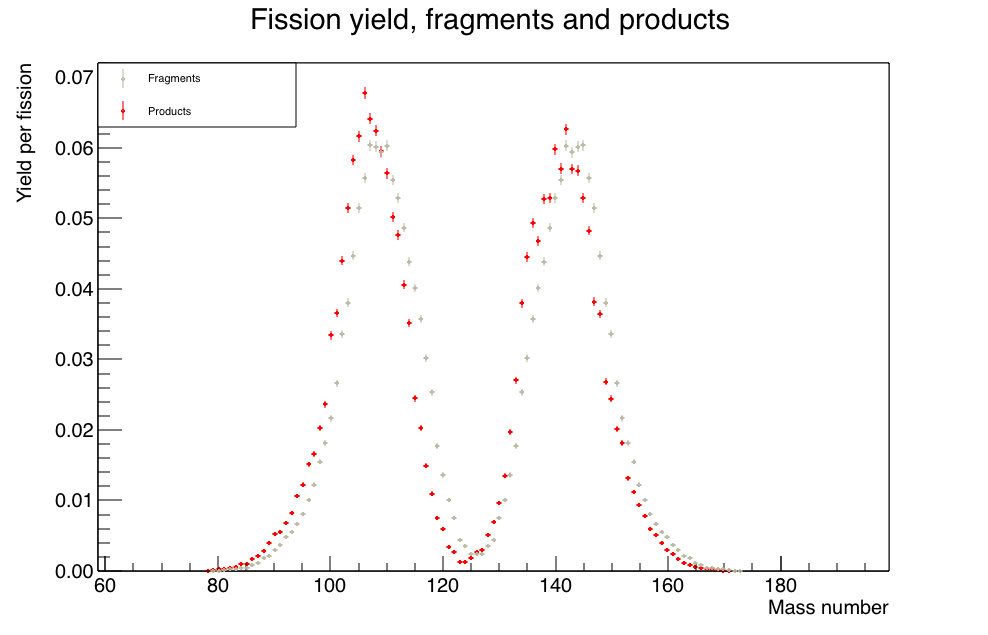
\includegraphics[scale=0.37]{Cf252_sf_fragment_product_yield.png}
	\caption{The fragment and product yield from the spontaneous fission of Cf252}
	\label{fig:Cf252_sf_fragment_product_yield}
\end{figure}

\begin{figure} [H]
	\centering
	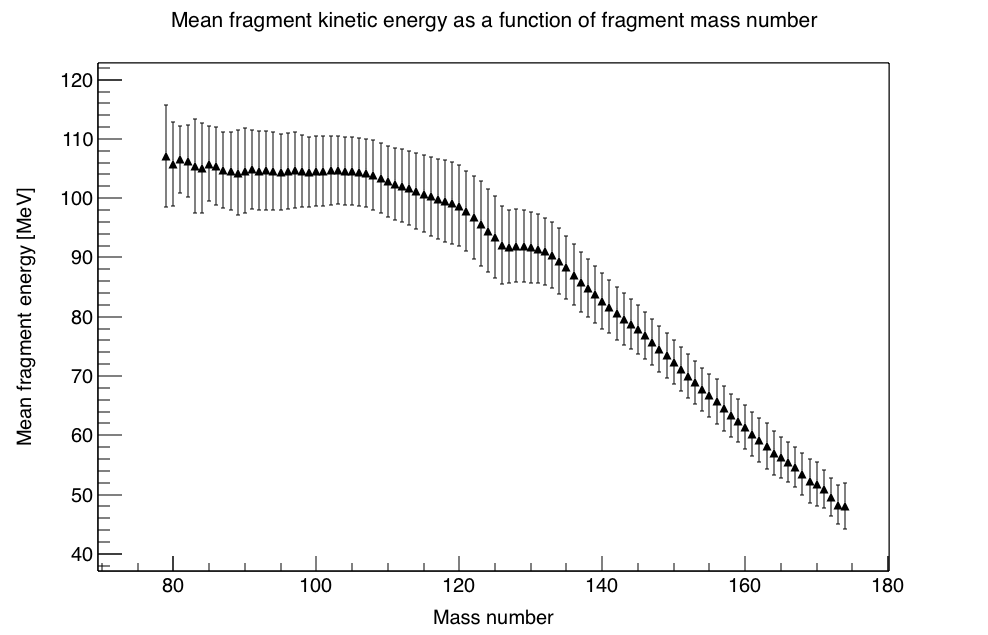
\includegraphics[scale=0.37]{Cf252_sf_mean_fragment_kinetic_enery_function_of_fragment_mass_number.png}
	\caption{The mean fragment energy as a function of fragment mass, from the spontaneous fission of Cf252}
	\label{fig:Cf252_sf_mean_fragment_kinetic_enery_function_of_fragment_mass_number}
\end{figure}

\begin{figure} [H]
	\centering
	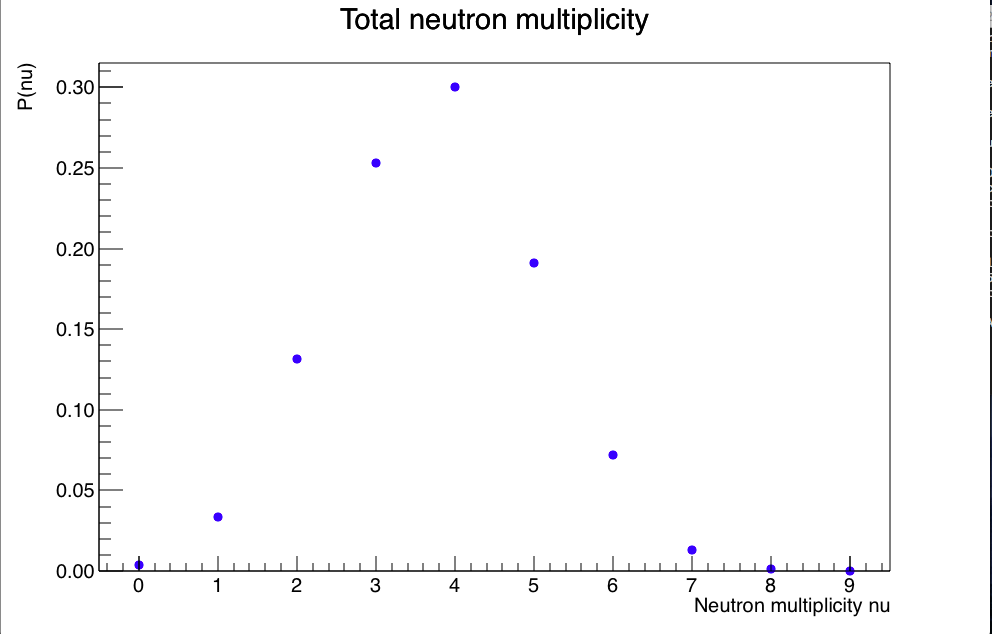
\includegraphics[scale=0.36]{Cf252_sf_total_n_mult.png}
	\caption{The multiplicity distribution of neutrons from the spontaneous fission of Cf252}
	\label{fig:Cf252_sf_total_n_mult}
\end{figure}

\begin{figure} [H]
	\centering
	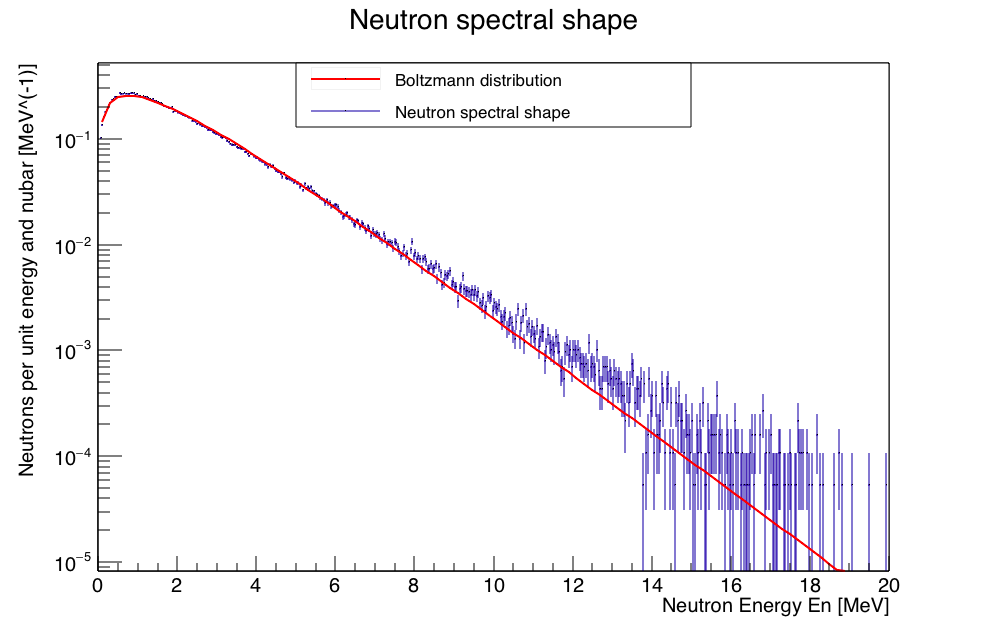
\includegraphics[scale=0.36]{Cf252_sf_neutron_spectral_shape.png}
	\caption{The spectral shape of neutrons from the spontaneous fission of Cf252, compared to a fitted Boltzmann distribution}
	\label{fig:Cf252_sf_neutron_spectral_shape}
\end{figure}

\begin{figure} [H]
	\centering
	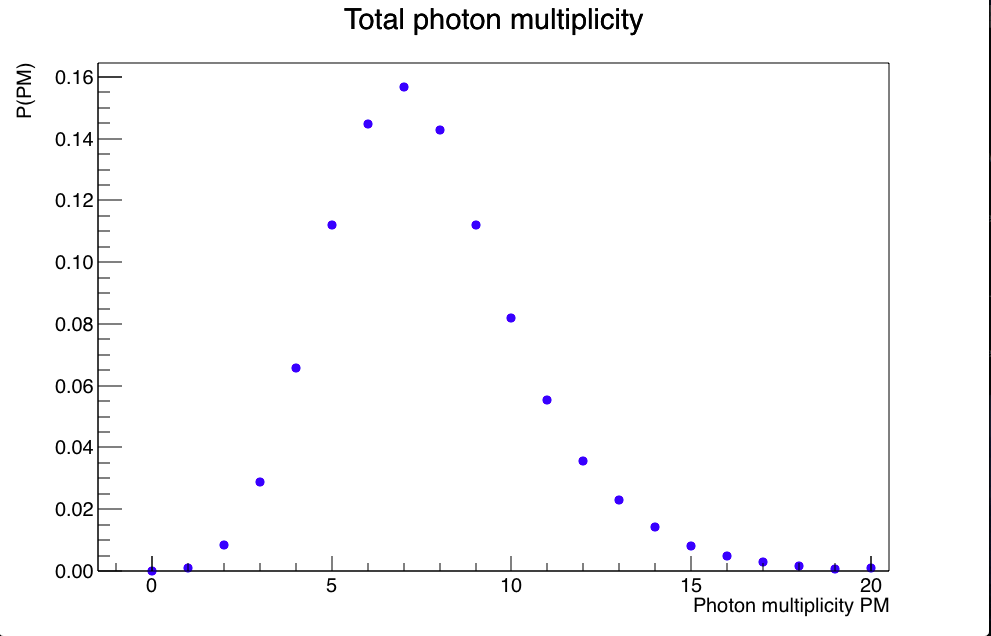
\includegraphics[scale=0.36]{Cf252_sf_total_ph_mult.png}
	\caption{The multiplicity distribution of photons from the spontaneous fission of Cf252}
	\label{fig:Cf252_sf_total_ph_mult}
\end{figure}

\begin{figure} [H]
	\centering
	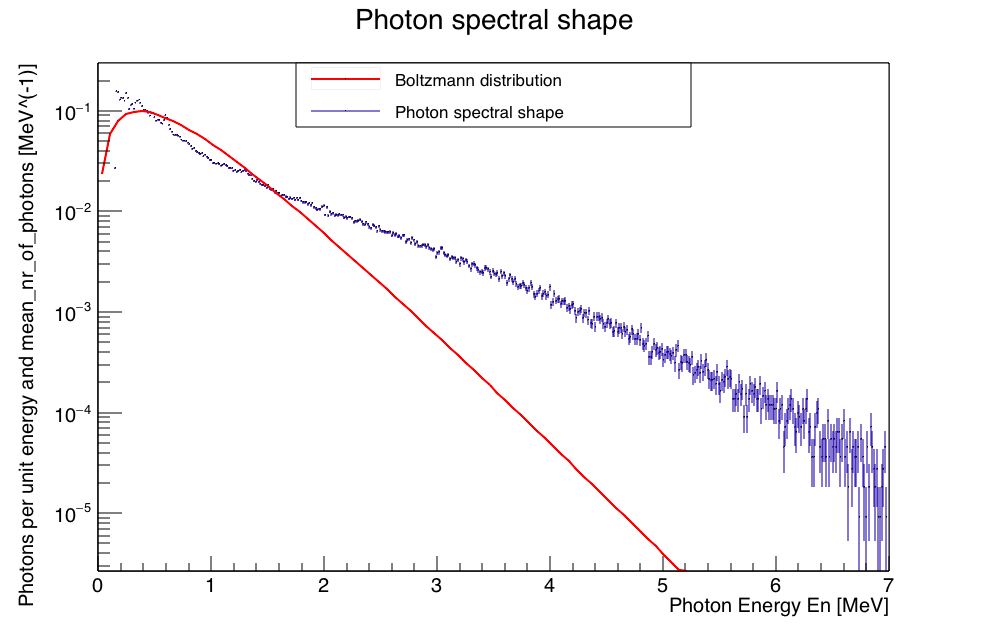
\includegraphics[scale=0.36]{Cf252_sf_photons_spectral_shape.png}
	\caption{The spectral shape of photons from the spontaneous fission of Cf252, compared to a fitted Boltzmann distribution}
	\label{fig:Cf252_sf_photons_spectral_shape}
\end{figure}
	
\begin{figure} [H]
	\centering
	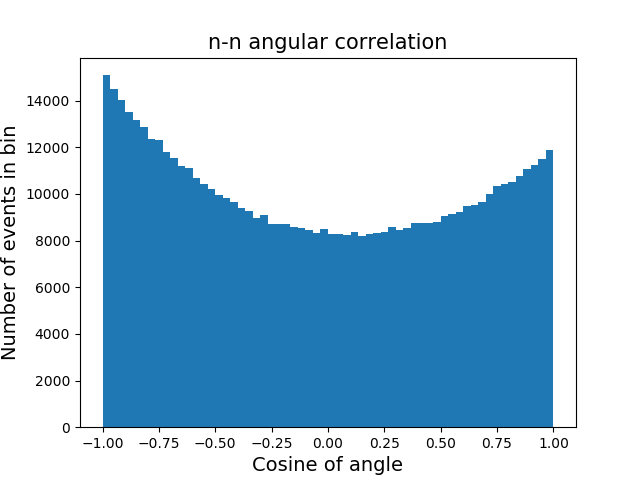
\includegraphics[scale=0.7]{Cf252_sf_n_n_ang_corr.png}
	\caption{The angulare correlation between pairs of emmited neutrons from the spontaneous fission of Cf252}
	\label{fig:Cf252_sf_n_n_ang_corr}
\end{figure}
	
\subsection{Thermal neutron induced fission of U235}

The four first neutron factorial moments is shown in table \ref{tab:U235_n_moments}. The fragment and product distribution is shown in Figure \ref{fig:U235_fragment_product_distribution}. 

The multiplicity distribution and spectral shape of the emmited neutrons and photons respectively is shown in Figure \ref{fig:U235_n_mult}, \ref{fig:U235_n_spectral_shape}, \ref{fig:U235_ph_mult} and \ref{fig:U235_ph_spectral_shape}. The angular correlation between pairs of emmited neutrons are shown in Figure \ref{fig:U235_n_n_ang_corr}.

\begin{table} [H]
	\centering
	\caption{Neutrons, first four factorial moments, from thermal neutron-induced fission of U235 }
	\begin{tabularx}{\textwidth}{XX} \hline
		\label{U235_n_moments}
		Moment & Value \\ \hline
		1 & 2.42969 \\
		2 & 4.66928\\
		3 & 6.7716\\
		4 & 7.01856\\ 
	\end{tabularx}
\end{table}

\begin{figure} [H]
	\centering
	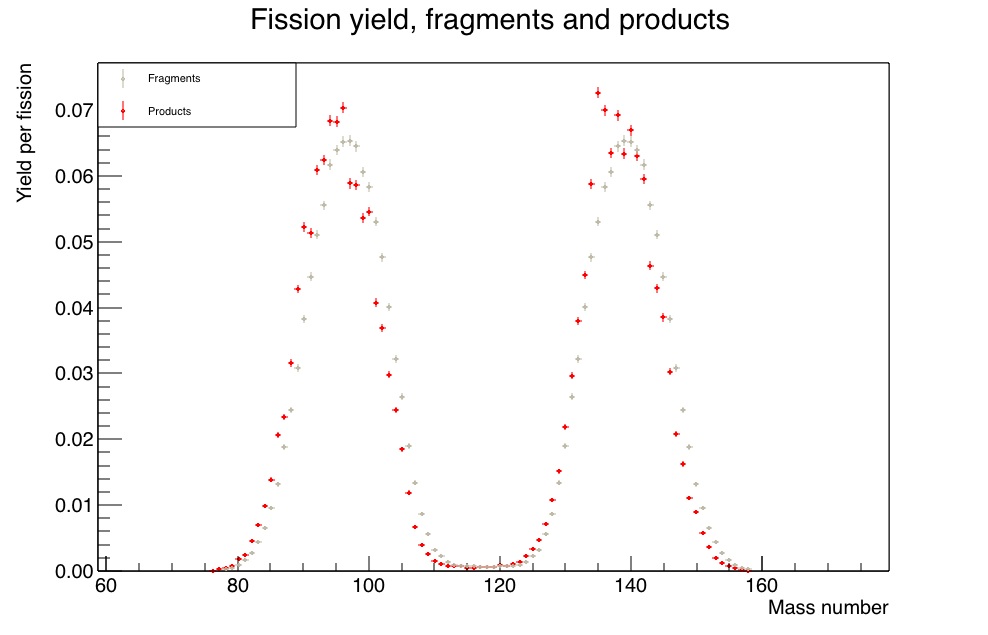
\includegraphics[scale=0.36]{U235_fragment_product_distribution.png}
	\caption{The fragment and product mass distribution from the thermal neutron induced fission of U235}
	\label{fig:U235_fragment_product_distribution}
\end{figure}

\begin{figure} [H]
	\centering
	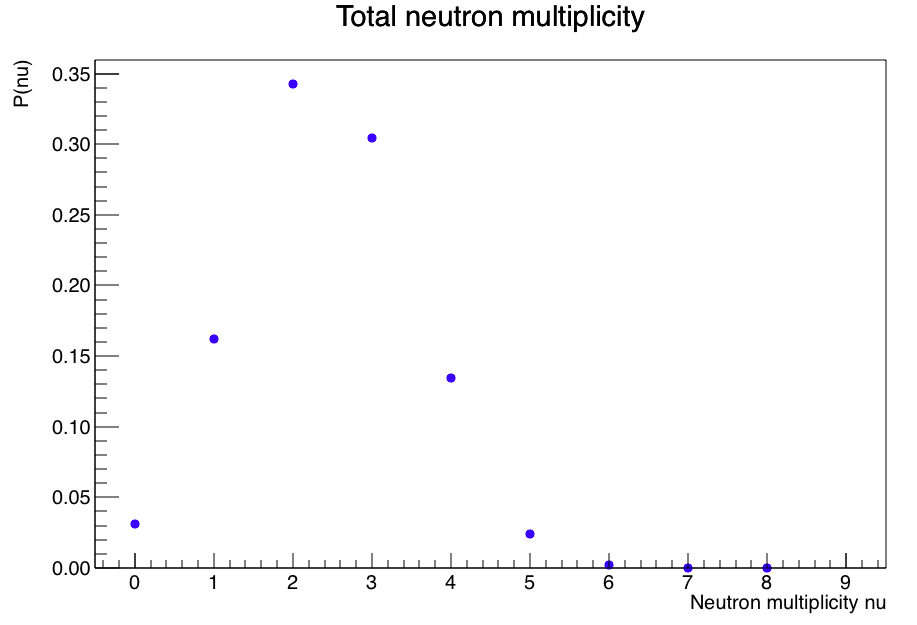
\includegraphics[scale=0.36]{U235_n_mult.png}
	\caption{The multiplicity distribution of neutrons from the thermal neutron-induced fission of U235}
	\label{fig:U235_n_mult}
\end{figure}

\begin{figure} [H]
	\centering
	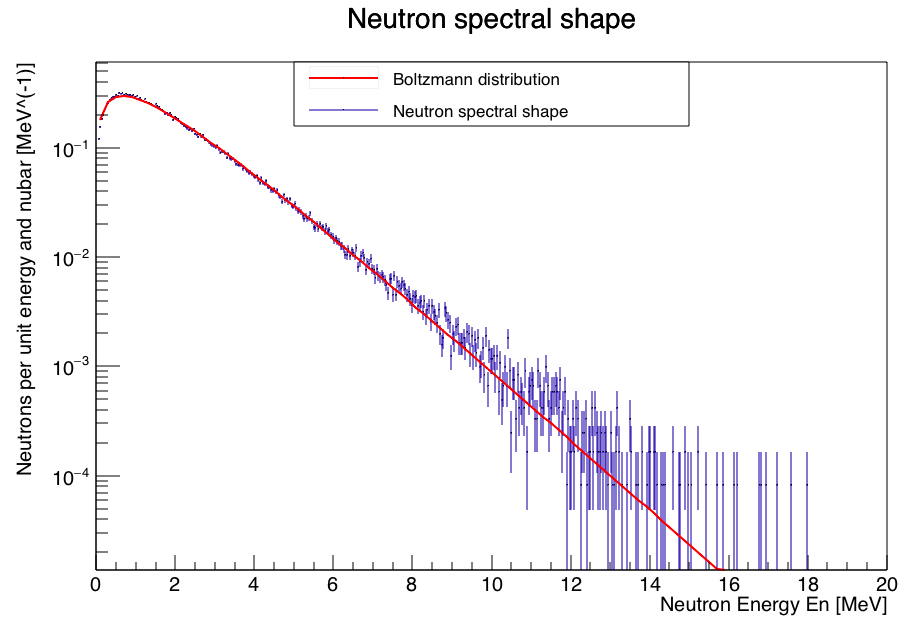
\includegraphics[scale=0.36]{U235_n_spectral_shape.png}
	\caption{The spectral shape of neutrons from the thermal neutron induced fission of U235, compared to a fitted Boltzmann distribution}
	\label{fig:U235_n_spectral_shape}
\end{figure}

\begin{figure} [H]
	\centering
	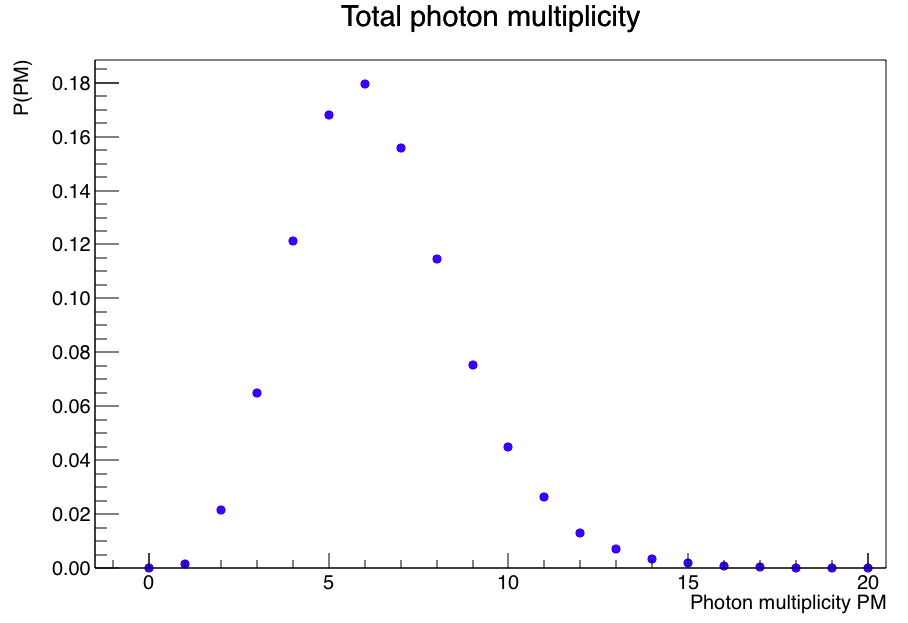
\includegraphics[scale=0.36]{U235_ph_mult.png}
	\caption{The multiplicity distribution of photons from the thermal neutron-induced fission of U235}
	\label{fig:U235_ph_mult}
\end{figure}

\begin{figure} [H]
	\centering
	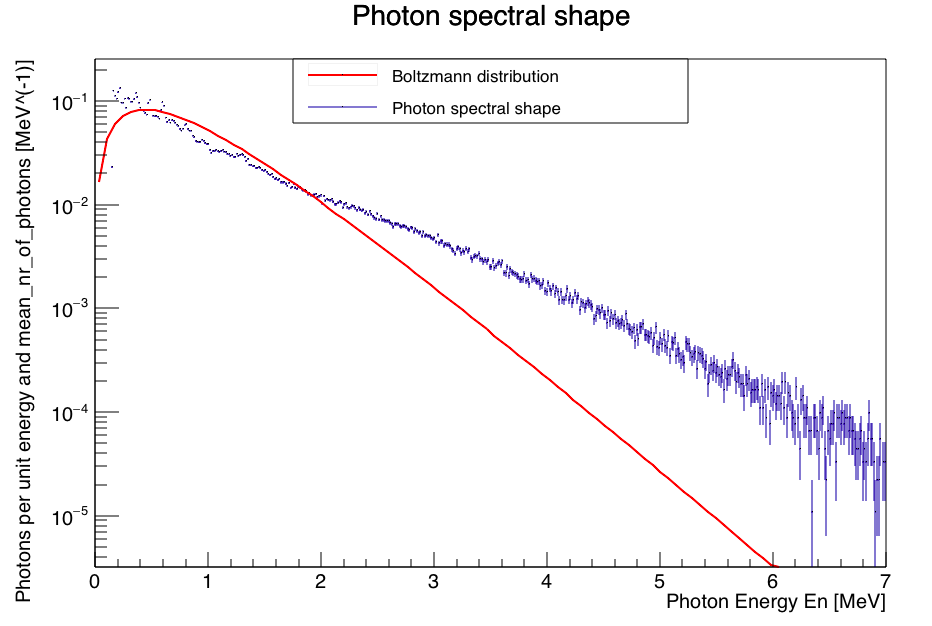
\includegraphics[scale=0.34]{U235_ph_spectral_shape.png}
	\caption{The spectral shape of photons from the thermal neutron induced fission of U235, compared to a fitted Boltzmann distribution}
	\label{fig:U235_ph_spectral_shape}
\end{figure}

\begin{figure} [H]
	\centering
	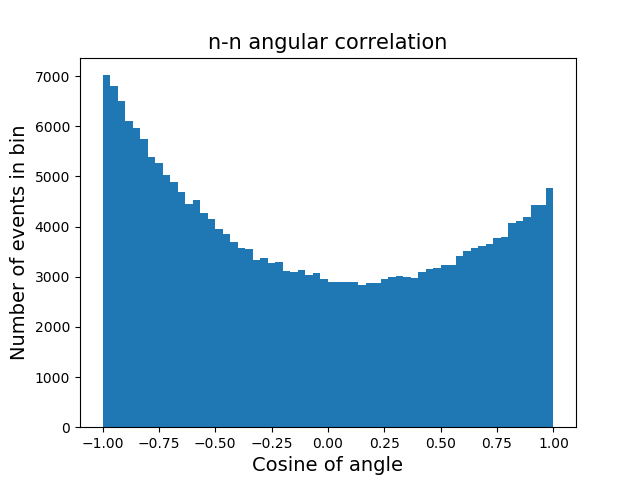
\includegraphics[scale=0.65]{U235_n_n_ang_corr.png}
	\caption{The angulare correlation between pairs of emmited neutrons from the thermal neutron-induced fission of U235}
	\label{fig:U235_n_n_ang_corr}
\end{figure}


\subsection{Neutron induced fission of Pu239}

\subsubsection{Neutron factorial moments for Pu239}

The first four neutron factorial moments for the neutron induced fission of Pu239 for incoming neutron energies $0.1, 2, 8, 14$ and $20$ MeV can be seen in Table \ref{tab:Pu239_n_moments_0_1} - \ref{tab:Pu239_n_moments_20}.

\begin{table} [H]
	\centering
	\caption{Neutrons, first four factorial moments. From neutron-induced fission of Pu239, with E$_n$ = 0.1 MeV }
	\begin{tabularx}{\textwidth}{XXXXX} \hline
		\label{tab:Pu239_n_moments_0_1}
		Moment & $\nu$ & $\nu_0$ & $\nu_1$ & $\nu_2$ \\ \hline
		1 & 2.89026 & 0 &1.62009 & 1.27017\\
		2 & 6.7476 & 0 & 1.75306 & 0.97784\\
		3 & 12.2142 & 0 & 1.07502 & 0.40332\\
		4 & 16.2727 & 0 & 0.29856 & 0.06936\\ 
	\end{tabularx}
\end{table}

\begin{table} [H]
	\centering
	\caption{Neutrons, first four factorial moments. From neutron-induced fission of Pu239, with E$_n$ = 2.0 MeV }
	\begin{tabularx}{\textwidth}{XXXXX} \hline
		\label{tab:Pu239_n_moments_2}
		Moment & $\nu$ & $\nu_0$ & $\nu_1$ & $\nu_2$ \\ \hline
		1 & 3.13967 & 0.00338 & 1.74664 & 1.39134\\
		2 & 8.12418 & 0 & 2.1249 & 1.24976\\
		3 & 16.7641 & 0 & 1.5852 & 0.65838\\
		4 & 26.4527 & 0 & 0.6012 & 0.18072\\ 
	\end{tabularx}
\end{table}

\begin{table} [H]
	\centering
	\caption{Neutrons, first four factorial moments. From neutron-induced fission of Pu239, with E$_n$ = 8.0 MeV }
	\begin{tabularx}{\textwidth}{XXXXX} \hline
		\label{tab:Pu239_n_moments_8}
		Moment & $\nu$ & $\nu_0$ & $\nu_1$ & $\nu_2$ \\ \hline
		1 & 3.8262 & 0.54674 & 1.97688 & 1.57595\\
		2 & 12.6219 & 0 & 2.9383 & 1.7681\\
		3 & 35.2788 & 0 & 3.09714 & 1.37334\\
		4 & 82.0861 & 0 & 2.2596 & 0.71616\\ 
	\end{tabularx}
\end{table}

\begin{table} [H]
	\centering
	\caption{Neutrons, first four factorial moments. From neutron-induced fission of Pu239, with E$_n$ = 14.0 MeV }
	\begin{tabularx}{\textwidth}{XXXXX} \hline
		\label{tab:Pu239_n_moments_14}
		Moment & $\nu$ & $\nu_0$ & $\nu_1$ & $\nu_2$ \\ \hline
		1 & 4.49802 & 0.93108 & 2.29912 & 1.73344\\
		2 & 18.217 & 0.48466 & 4.32362 & 2.2436\\
		3 & 65.9636 & 0 & 6.57924 & 2.13492\\
		4 & 212.075 & 0 & 8.1756 & 1.45224\\ 
	\end{tabularx}
\end{table}

\begin{table} [H]
	\centering
	\caption{Neutrons, first four factorial moments. From neutron-induced fission of Pu239, with E$_n$ = 20.0 MeV }
	\begin{tabularx}{\textwidth}{XXXXX} \hline
		\label{tab:Pu239_n_moments_20}
		Moment & $\nu$ & $\nu_0$ & $\nu_1$ & $\nu_2$ \\ \hline
		1 & 5.04612 & 1.11361 & 2.57681 & 1.91351\\
		2 & 23.3884 & 0.72198 & 5.61242 & 2.83246\\
		3 & 98.8097 & 0.04158 & 10.1763 & 3.16566\\
		4 & 377.024 & 0 & 15.2033 & Moment4 2.58768\\ 
	\end{tabularx}
\end{table}

\subsubsection{Fragment and product mass distributions}

The fragment and product distribution from the neutron-induced fission of Pu239 for incoming neutron energies $E_n=$ 0.1, 8 and 20 MeV is shown in Figure \ref{fig:Pu239_0_1_fragment_product}, \ref{fig:Pu239_8_fragment_product}, \ref{fig:Pu239_20_fragment_product}.

\begin{figure} [H]
	\centering
	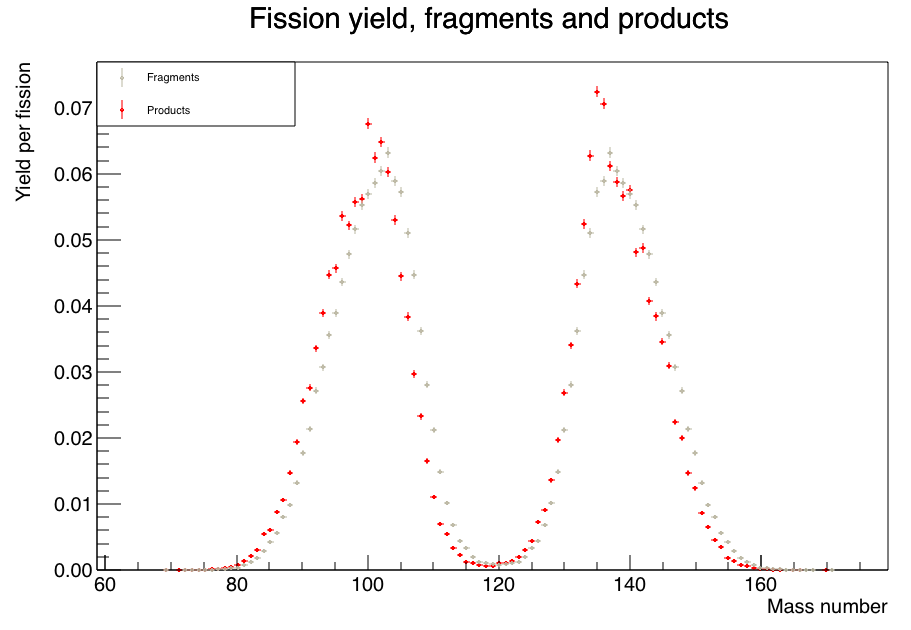
\includegraphics[scale=0.36]{Pu239_0_1_fragment_product.png}
	\caption{The fragment and product distribution from the neutron-induced fission of Pu239 with $E_n = 0.1$ MeV}
	\label{fig:Pu239_0_1_fragment_product}
\end{figure}

\begin{figure} [H]
	\centering
	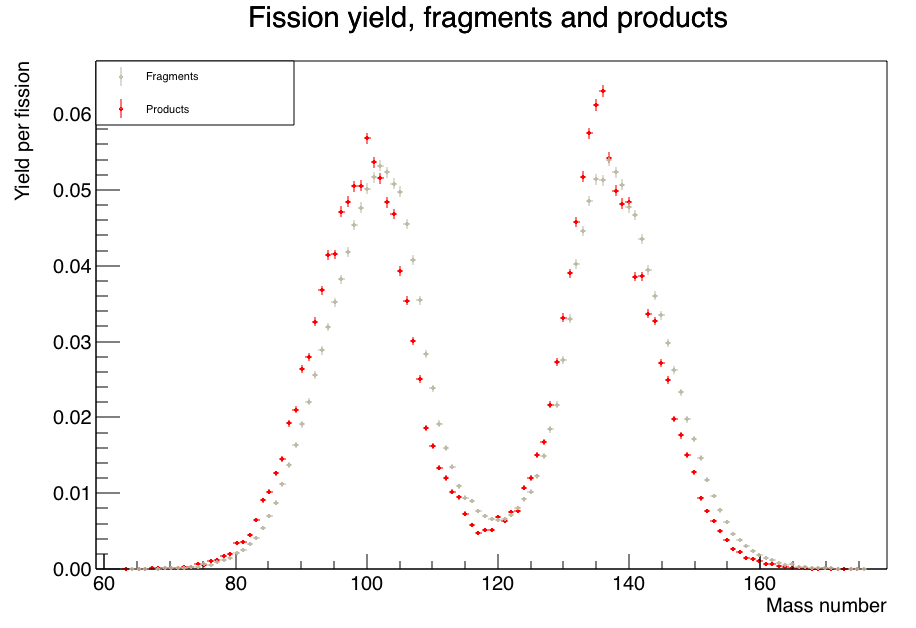
\includegraphics[scale=0.36]{Pu239_8_fragment_product.png}
	\caption{The fragment and product distribution from the neutron-induced fission of Pu239 with $E_n = 8$ MeV}
	\label{fig:Pu239_8_fragment_product}
\end{figure}

\begin{figure} [H]
	\centering
	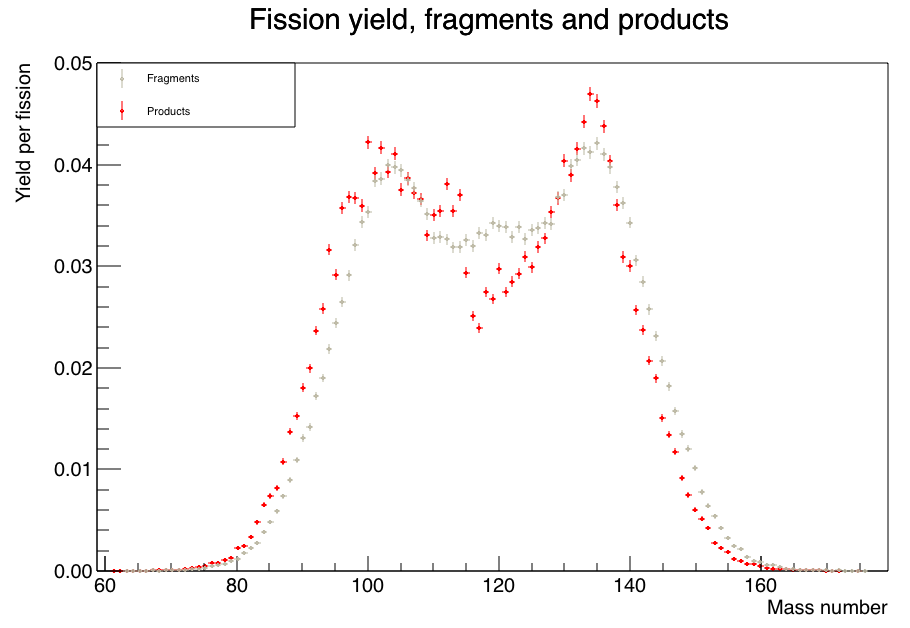
\includegraphics[scale=0.36]{Pu239_20_fragment_products.png}
	\caption{The fragment and product distribution from the neutron-induced fission of Pu239 with $E_n = 20$ MeV}
	\label{fig:Pu239_20_fragment_product}
\end{figure}

\subsubsection{Neutron multiplicity distribution and spectral shape}

The neutron multiplicity distribution for the neutron-induced fission of Pu239 for the incoming neutron energies $E_n$ = 0.1, 8 and 20 MeV is shown in Figure \ref{fig:Pu239_0_1_n_mult}, \ref{fig:Pu239_8_n_mult} and \ref{fig:Pu239_20_n_mult}.

The spectral shapes of the same incoming neutron energies are shown in Figure \ref{fig:Pu239_0_1_n_spectral_shape}, \ref{fig:Pu239_8_n_spectral_shape} and \ref{fig:Pu239_20_n_spectral_shape}.

\begin{figure} [H]
	\centering
	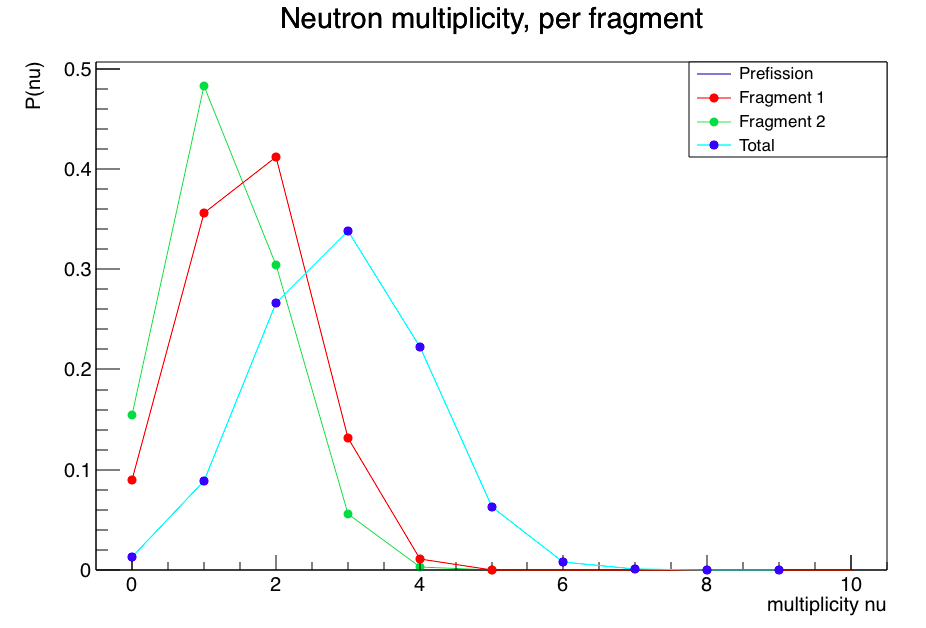
\includegraphics[scale=0.36]{Pu239_0_1_n_mult.png}
	\caption{The neutron multiplicity distribution from the neutron-induced fission of Pu239 with $E_n = 0.1$ MeV}
	\label{fig:Pu239_0_1_n_mult}
\end{figure}

\begin{figure} [H]
	\centering
	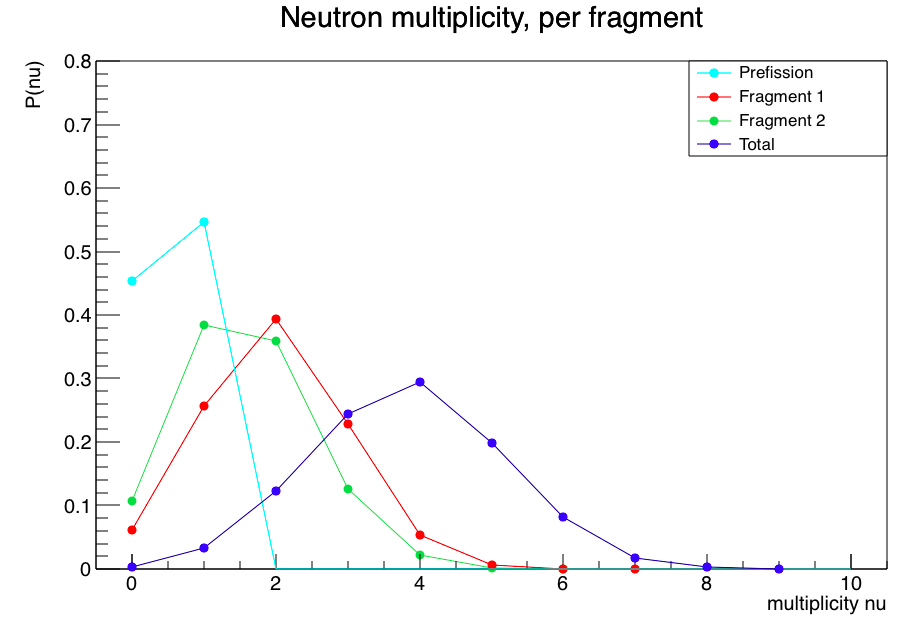
\includegraphics[scale=0.36]{Pu239_8_n_mult.png}
	\caption{The neutron multiplicity distribution from the neutron-induced fission of Pu239 with $E_n = 8$ MeV}
	\label{fig:Pu239_8_n_mult}
\end{figure}

\begin{figure} [H]
	\centering
	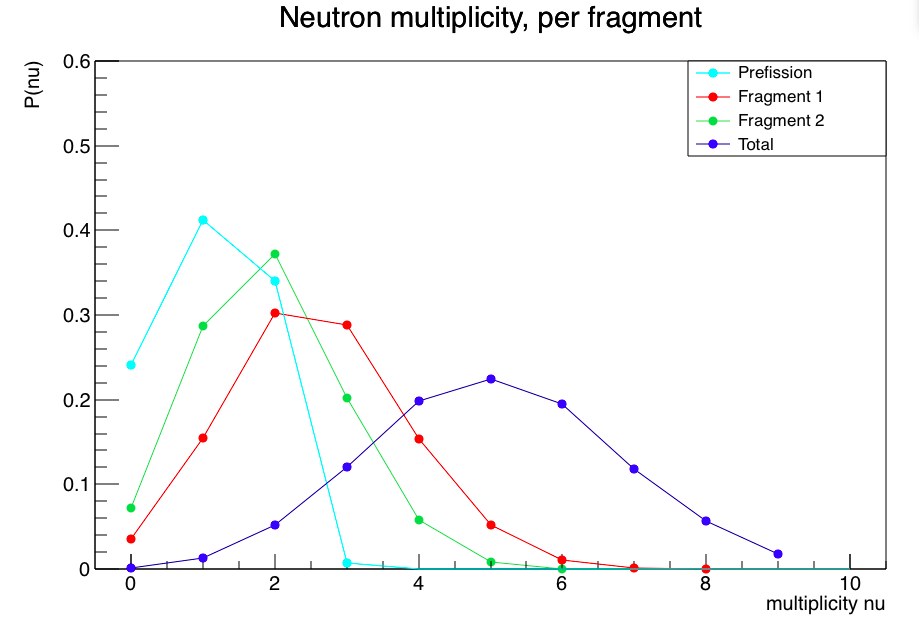
\includegraphics[scale=0.36]{Pu239_20_n_mult.png}
	\caption{The neutron multiplicity distribution from the neutron-induced fission of Pu239 with $E_n = 20$ MeV}
	\label{fig:Pu239_20_n_mult}
\end{figure}

\begin{figure} [H]
	\centering
	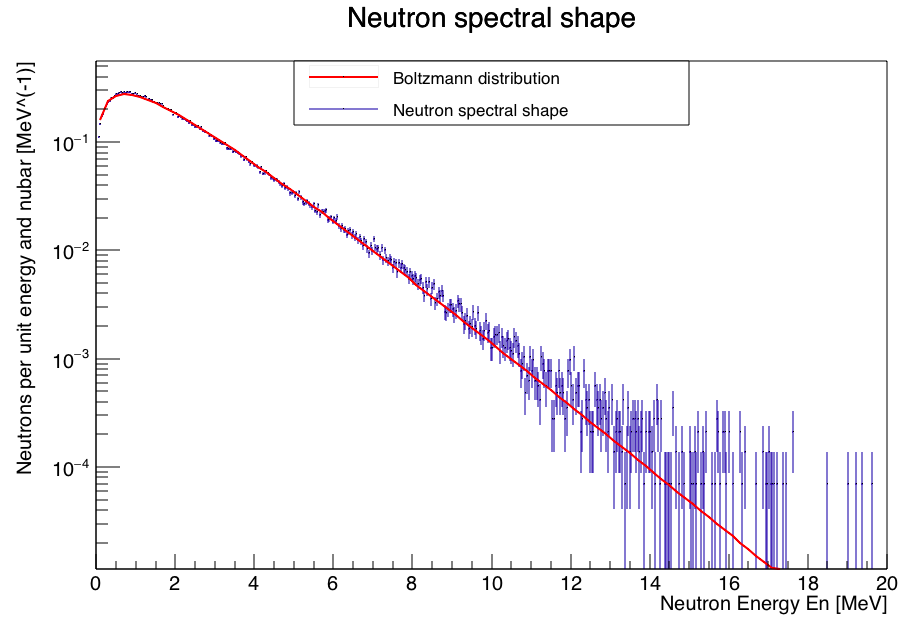
\includegraphics[scale=0.36]{Pu239_0_1_n_spectral_shape.png}
	\caption{The neutron spectral shape from the neutron-induced fission of Pu239 with $E_n = 0.1$ MeV, compared to a Boltzmnn distribution}
	\label{fig:Pu239_0_1_n_spectral_shape}
\end{figure}

\begin{figure} [H]
	\centering
	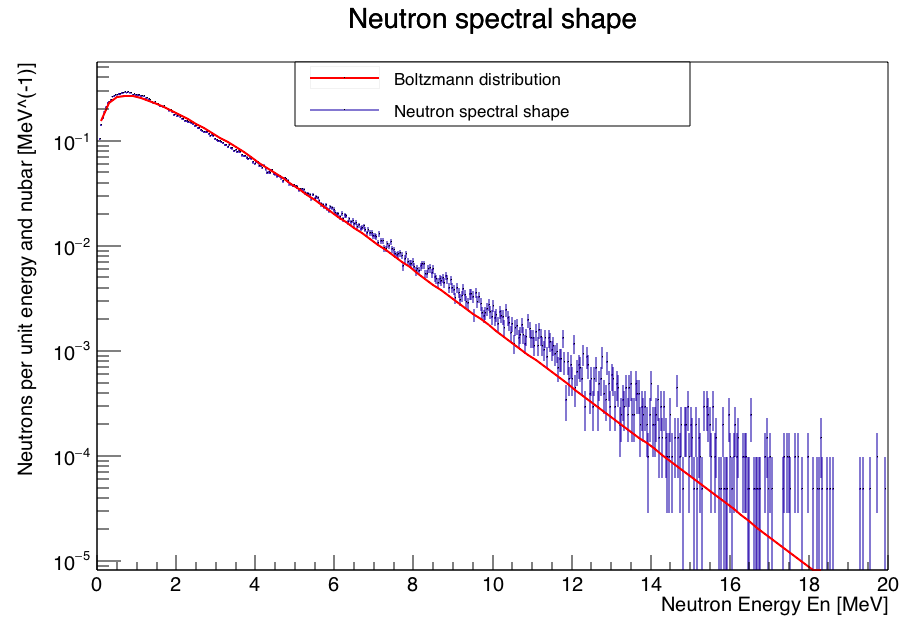
\includegraphics[scale=0.36]{Pu239_8_n_spectral_shape.png}
	\caption{The neutron spectral shape from the neutron-induced fission of Pu239 with $E_n = 8$ MeV, compared to a Boltzmnn distribution}
	\label{fig:Pu239_8_n_spectral_shape}
\end{figure}

\begin{figure} [H]
	\centering
	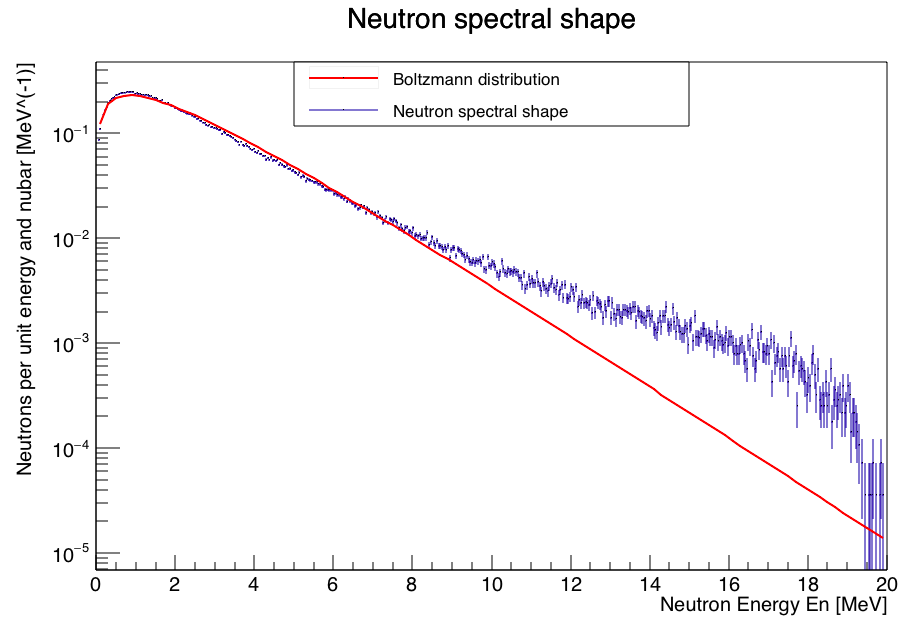
\includegraphics[scale=0.36]{Pu239_20_n_spectral_shape.png}
	\caption{The neutron spectral shape from the neutron-induced fission of Pu239 with $E_n = 20$ MeV, compared to a Boltzmnn distribution}
	\label{fig:Pu239_20_n_spectral_shape}
\end{figure}

\subsubsection{Photon multiplicity distribution and spectral shape}

The photon multiplicity distribution for the neutron-induced fission of Pu239 for the incoming neutron energies $E_n$ = 0.1, 8 and 20 MeV is shown in Figure \ref{fig:Pu239_0_1_ph_mult}, \ref{fig:Pu239_8_ph_mult} and \ref{fig:Pu239_20_ph_mult}.

The spectral shapes of the same incoming neutron energies are shown in Figure \ref{fig:Pu239_0_1_ph_spectral_shape}, \ref{fig:Pu239_8_ph_spectral_shape} and \ref{fig:Pu239_20_ph_spectral_shape}.

\begin{figure} [H]
	\centering
	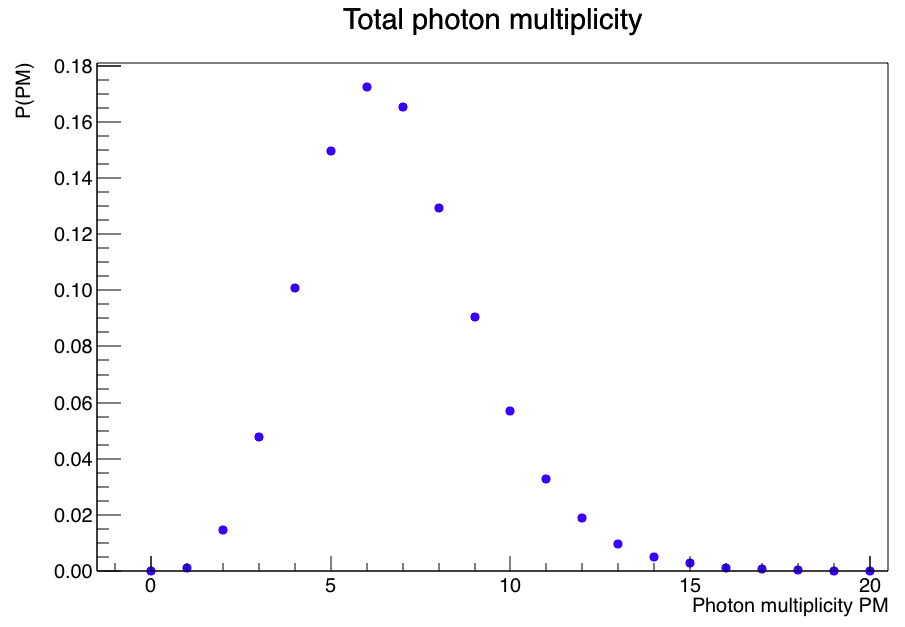
\includegraphics[scale=0.36]{Pu239_0_1_ph_mult.png}
	\caption{The photon multiplicity distribution from the neutron-induced fission of Pu239 with $E_n = 0.1$ MeV}
	\label{fig:Pu239_0_1_ph_mult}
\end{figure}

\begin{figure} [H]
	\centering
	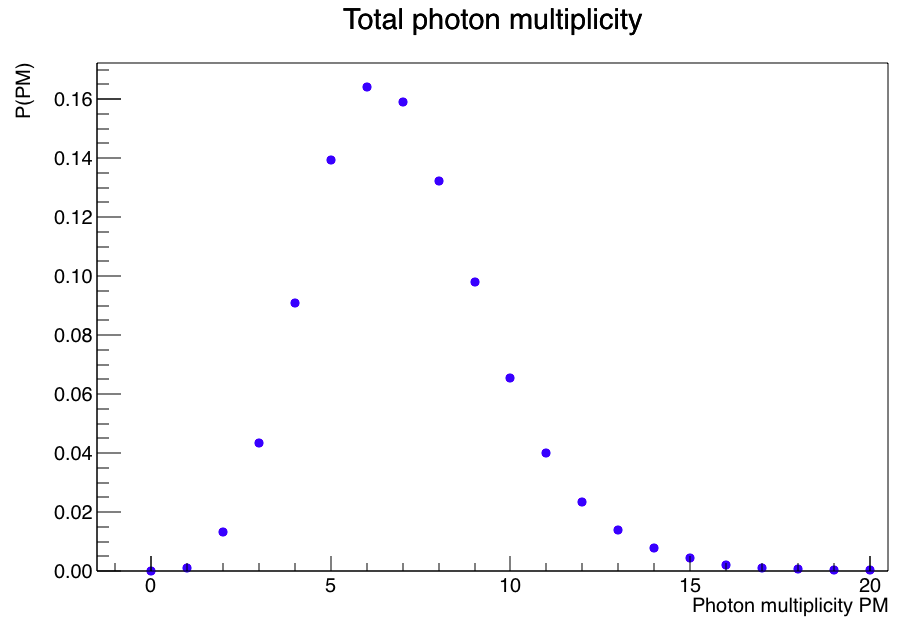
\includegraphics[scale=0.36]{Pu239_8_ph_mult.png}
	\caption{The photon multiplicity distribution from the neutron-induced fission of Pu239 with $E_n = 8$ MeV}
	\label{fig:Pu239_8_ph_mult}
\end{figure}

\begin{figure} [H]
	\centering
	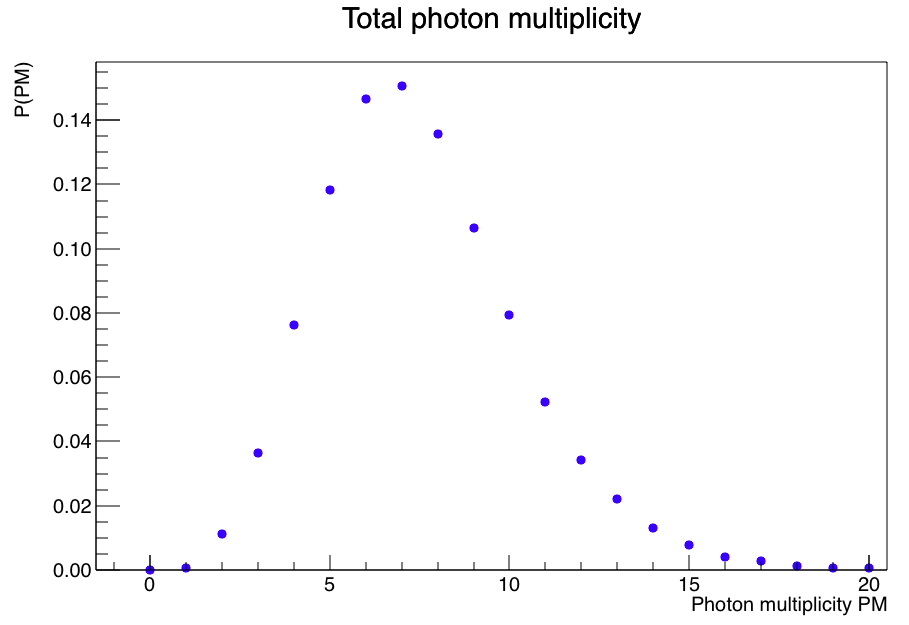
\includegraphics[scale=0.36]{Pu239_20_ph_mult.png}
	\caption{The photon multiplicity distribution from the neutron-induced fission of Pu239 with $E_n = 20$ MeV}
	\label{fig:Pu239_20_ph_mult}
\end{figure}

\begin{figure} [H]
	\centering
	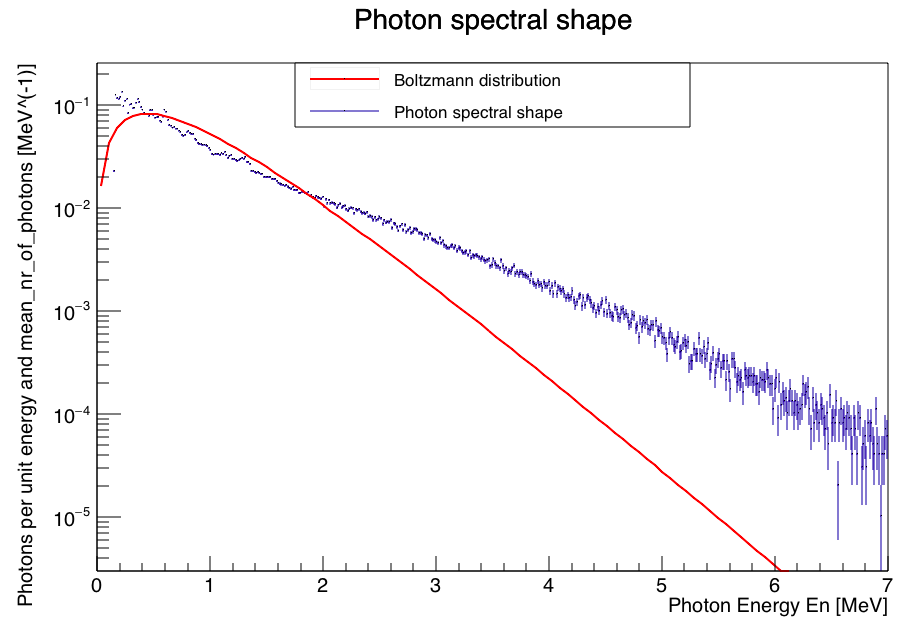
\includegraphics[scale=0.36]{Pu239_0_1_ph_spectral_shape.png}
	\caption{The photon spectral shape from the neutron-induced fission of Pu239 with $E_n = 0.1$ MeV, compared to a Boltzmnn distribution}
	\label{fig:Pu239_0_1_ph_spectral_shape}
\end{figure}

\begin{figure} [H]
	\centering
	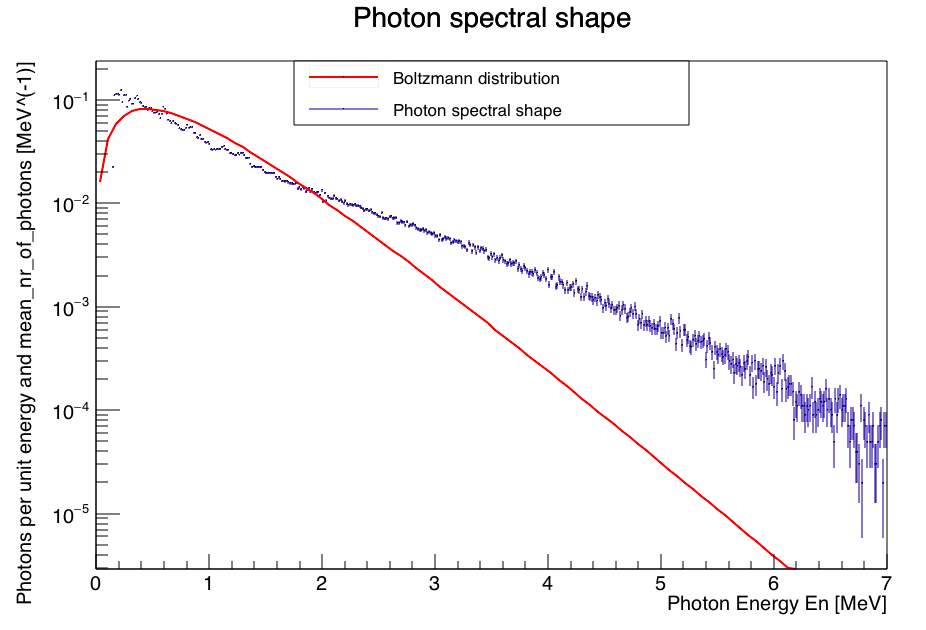
\includegraphics[scale=0.36]{Pu239_8_ph_spectral_shape.png}
	\caption{The photon spectral shape from the neutron-induced fission of Pu239 with $E_n = 8$ MeV, compared to a Boltzmnn distribution}
	\label{fig:Pu239_8_ph_spectral_shape}
\end{figure}

\begin{figure} [H]
	\centering
	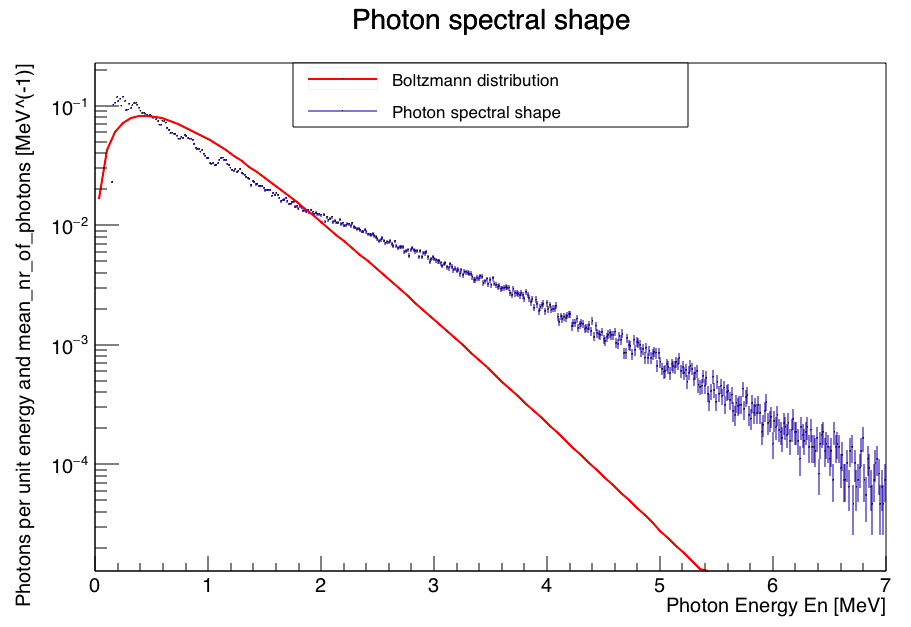
\includegraphics[scale=0.36]{Pu239_20_ph_spectral_shape.png}
	\caption{The photon spectral shape from the neutron-induced fission of Pu239 with $E_n = 20$ MeV, compared to a Boltzmnn distribution}
	\label{fig:Pu239_20_ph_spectral_shape}
\end{figure}

\subsubsection{Angular correlation of neutron pairs}
The angular correlation between pair of emmited neutrons for the incoming neutron energies $E_n =$ 0.1, 8 and 20 MeV are shown in Figure

\begin{figure} [H]
	\centering
	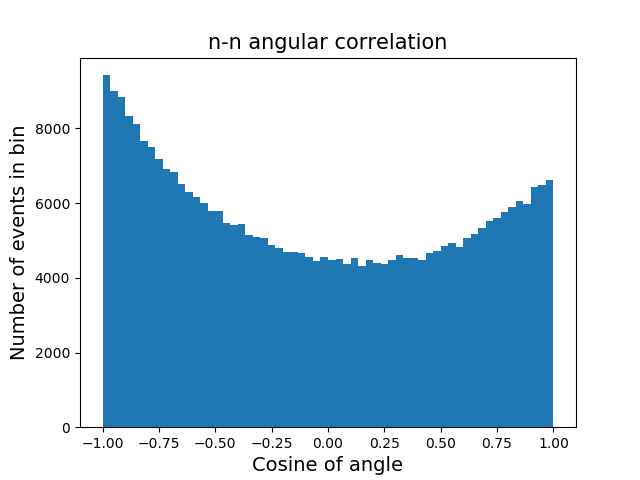
\includegraphics[scale=0.65]{Pu239_0_1_n_n_ang_corr.png}
	\caption{The angulare correlation between pairs of emmited neutrons from the neutron-induced fission of Pu239 with $E_n= 0.1$ MeV}
	\label{fig:Pu239_0_1_n_n_ang_corr}
\end{figure}

\begin{figure} [H]
	\centering
	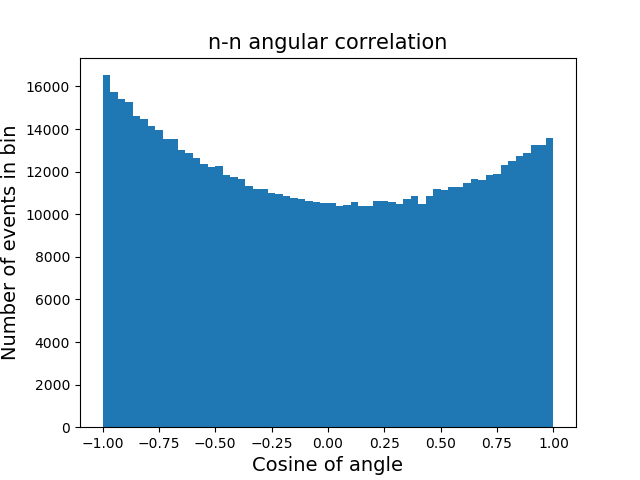
\includegraphics[scale=0.65]{Pu239_8_n_n_ang_corr.png}
	\caption{The angulare correlation between pairs of emmited neutrons from the neutron-induced fission of Pu239 with $E_n= 8$ MeV}
	\label{fig:Pu239_8_n_n_ang_corr}
\end{figure}

\begin{figure} [H]
	\centering
	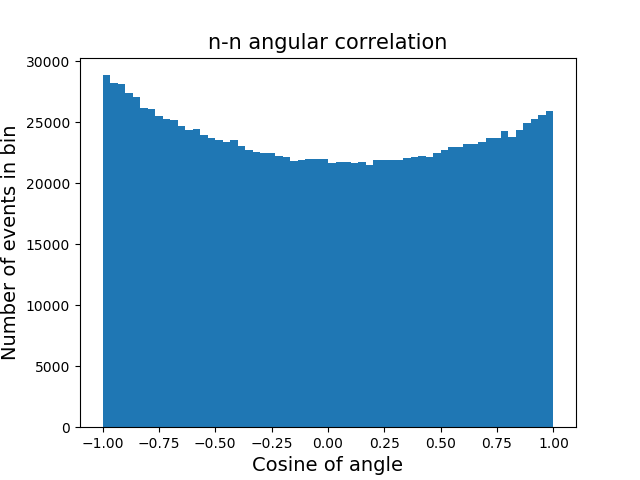
\includegraphics[scale=0.65]{Pu239_20_n_n_ang_corr.png}
	\caption{The angulare correlation between pairs of emmited neutrons from the neutron-induced fission of Pu239 with $E_n= 20$ MeV}
	\label{fig:Pu239_20_n_n_ang_corr}
\end{figure}

\section{Discussion}

From Table \ref{tab:dependence_on_dTKE}, I see that both the mean neutron multiplicity $\nu$ and the mean gamma multiplicity $N_{\gamma}$ decreases as dTKE increases. As explained in section \ref{Parameters_FREYA}, dTKE decides how the available energy is partitioned between the kinetic energy and the excitation energy of the nucelus. As dTKE increases, less of the energy is put as excitation energy. As both neutron emission and gamma emission requires excitation energy from the nucleus, these average multiplicity of these decreases.\par 
\vspace{3mm}

Furthermore, Table \ref{tab:dependence_on_x} shows that for higher x, the average neutron mutiplicity from the light fission fragment $\nu_1$ increases, while the neutron muntiplicity from the heavy fission fragment $\nu_2$ decreases. This is as expected. The parameter x shifts the distribution of excitation energy between the two fission fragments in the light fission fragment's favour. The more excitation energy available, the more neutrons can the nucelus emit, as the nuceus must have more excitation energy than the neutron separation energy $S_n$ to emit a neutron. Therefore, $\nu_1$ increases while $\nu_2$ decreases. \par 
\vspace{3mm}

From Table \ref{tab:dependence_on_c}, I see that the average gamma multiplicity $N_{\gamma}$ increases as c infreases. As explained in section \ref{Parameters_FREYA}, c is the so-called spin temperature, that effectively desides how much of the excitation energy should be rotational energy, compared to statistical excitation energy. As neutron emission more or less conserves its own angular momentum during neutron emission, the total angular momentum of the nucleus remains unchanged, and thus neutron emission only strips the nucleus of statistical excitation energy. After neutron emission is no longer possible, the nucleus rids itself of rotational excitation energy through the emission of photons. Therefore, the more energy available as rotational excitation energy in the nucleus, the higher the average gamma multiplicity $N_{\gamma}$ will be, and this is in accordance with Table \ref{tab:dependence_on_c}.
\par 
\vspace{3mm}

As can be seen from Figure \ref{fig:Pu239_0_1_fragment_product}, \ref{fig:Pu239_8_fragment_product} and \ref{fig:Pu239_20_fragment_product}, in neutron induced fission, the fragment mass distribution changes with the energy of the incoming energy. For low incoming neutron energies, the fission fragment distribution has two separate humps for low and high frament mass respectively, while for larger incomning neutron energies the two humps becomes more and more like a one hump distribution. The reason why, is that for low compound nucleus energies, shell effects play a large role in determining the fission fragments. When one of the fission fragments have neutron or proton numbers which correspond to magic numbers, where the nuckeus is especially bound, more energy is released. For higher incoming neutron energies, however, the compound nucleus have a higher excitation energy, and therefore shell effects are less prominent. This can be seen when the two fission fragment distribution humps merge into one hump for large incoming neutron energies.\par 
\vspace{3mm}

In Figure \ref{fig:Pu239_0_1_n_n_ang_corr}, \ref{fig:Pu239_8_n_n_ang_corr} and \ref{fig:Pu239_20_n_n_ang_corr}, I observe that the angular correlation between pairs of emmited neutrons after neutron induced fission become less prominent for high incoming neutron energies. The neutrons are emmited in the fission fragment's rest system, and in this system, the neutrons are emitted isotropically. However, due to the kinetic energy of the fission fragment, the neutrons get a boost in the direction of the velocity of the fission fragments, when observed from the lab system. For lower energy neutrons, this boost is prominent, and as all the neutrons get this boost, there is a strong angular correlation between the emitted neutrons in the lab system. For higher incoming neutron energies, more excitation energy is availible when the neutrons are emmited, and they have a higher velocity. This velocity is not negligle comparet to the kinetic energy of the fission fragment, and thus the angular correlation between the emmited neutrons are less prominent.


\section{Conclusion}

\vspace{3mm}

\bibliographystyle{plain}
\bibliography{FREYA.bib}

\end{document} 

